\documentclass[a4paper, titlepage]{report}

\usepackage[francais]{babel}
\usepackage[utf8]{inputenc}
\usepackage[T1]{fontenc}

\usepackage{listings}
\usepackage{titlesec}
\usepackage{color}
\usepackage{graphicx}

\titleformat{\chapter}[display]
  {\bfseries\Large}
  {\filright\textsc{\chaptertitlename} \LARGE\thechapter}
  {1ex}
  {\titlerule\vspace{1ex}\filleft}
  [\vspace{1ex}\titlerule]


\definecolor{gris}{rgb}{0.97,0.97,0.97}
\definecolor{vert}{rgb}{0,0.6,0}
\definecolor{mauve}{rgb}{0.5,0,0.5}
\definecolor{rose}{rgb}{1,0.5,1}
\definecolor{cyan}{rgb}{0.1,0.4,0.6}
\definecolor{marron}{rgb}{0.4,0.2,0}
\definecolor{jaune}{rgb}{1,0.6,0}
\definecolor{bleu}{rgb}{0,0,0.8}

\lstset{
	language=R,	
	frame=tblr,
	numbers=left,
	breaklines=true,
	backgroundcolor=\color{gris},
    basicstyle=\small\ttfamily,
    stringstyle=\color{vert},
    otherkeywords={0,1,2,3,4,5,6,7,8,9},
    morekeywords={TRUE,FALSE},
    deletekeywords={data,frame,length,as,character},
    keywordstyle=\color{blue},
    commentstyle=\color{vert},
}


\title{Rapport Projet SY09}
\date{3 mai 2018}
\author{Yiqing \textsc{Su} et Théophile \textsc{Molcard}}


\begin{document}

\renewcommand{\chaptername}{Partie}


\maketitle

\tableofcontents



\chapter{Cuisine}

Le jeu de données à étudier de la première partie est un ensemble de recettes de cuisine de diverses origines.\\
\indent Pour la question de 1.1 jusqu'à 1.5, le jeu de données utilisé est une version agrégée par origine. Puis pour les restes questions, il s'agit d'utiliser les données sans agrégation, autrement dit, il y a toutes les recettes de chaque pays ou région.

\section{Analyse exploratoire}
Le premier jeu de données comporte 26 lignes et 51 colonnes. Une ligne représente des informations synthétiques d'une recette pour un pays ou une région. Puis la première colonne indique le nom du pays ou de la région et les autres colonnes représentent l'utilisation des 50 ingrédients dans la recette. Les pays et les régions indiqués dans ces données sont asiatiques, européens ou américains.\\
\indent Avec \textbf{boxplot} et \textbf{summary}, nous pouvons voir que les données sont toutes entre 0 et 1. La moyenne pour chaque boîte à moustache est inférieur à 0,5. Parmi tous les pays ou régions, il y a plus que deux tiers qui ne sont pas asiatiques. Donc, les ingrédients comme "olive oil" et "cayenne" ont plus de variances parce que certains recettes utilisent beaucoup cet ingrédient et les autres non. Les ingrédients comme "soy sauce" et "sesame oil" sont faibles à la moyenne et à la variance parce que seulement les pays et les régions asiatiques vont les utiliser.\\
\indent Nous nous intéressons par la corrélation entre les données. Figure 1.1 et Figure 1.2 montrent la corrélation de manière que plus la couleur est foncé, plus la corrélation est forte. Dans Figure 1.1, nous pouvons voir qu'il y a beaucoup d'ingrédients corrélés entre eux et il y a une partie de corrélations fortes. Plus précisément, en calculant la proportion nous savons que les coefficients de corrélation qui sont plus que 0.3 ont pris une partie presque un moitié (47.2\%). Dans Figure 1.2, nous pouvons voir clairement qu'il existe beaucoup de relations entre les données. Il semble normal parce que nous avons vu que les recettes de pays viennent principalement la région asiatique, la région européenne et la région américaine.
\begin{figure}[htbp]
\centering
\begin{minipage}[t]{0.5\textwidth}
\centering
\includegraphics[width=6.5cm]{./doc/plot-correlation-cuisine1.png}
\caption{Corrélation entre les ingrédients}
\end{minipage}
\begin{minipage}[t]{0.48\textwidth}
\centering
\includegraphics[width=5cm]{./doc/plot-correlation-cuisine1_2.png}
\caption{Corrélation entre les recettes de pays}
\end{minipage}
\end{figure}


\section{Analyse en composantes principales}
La matrice que l'on étudie est de dimension $M_{26,50}$, elle est donc de rang inférieur à 26. L'inertie peut donc être entièrement expliquée par 26 composantes. En effectuant une ACP sur ces données on obtient donc les 26 composantes principales expliquant l'inertie du nuage de points. Si l'on cherche les valeurs propres de la matrice de covariance, on constate comme attendu que 24 des valeurs propres qui résultent sont nulles.\\

\newpage
On peut donc afficher l'inertie expliquée par chaque composantes et par la somme des n premiers axes.
\begin{figure}[h]
	\begin{center}
		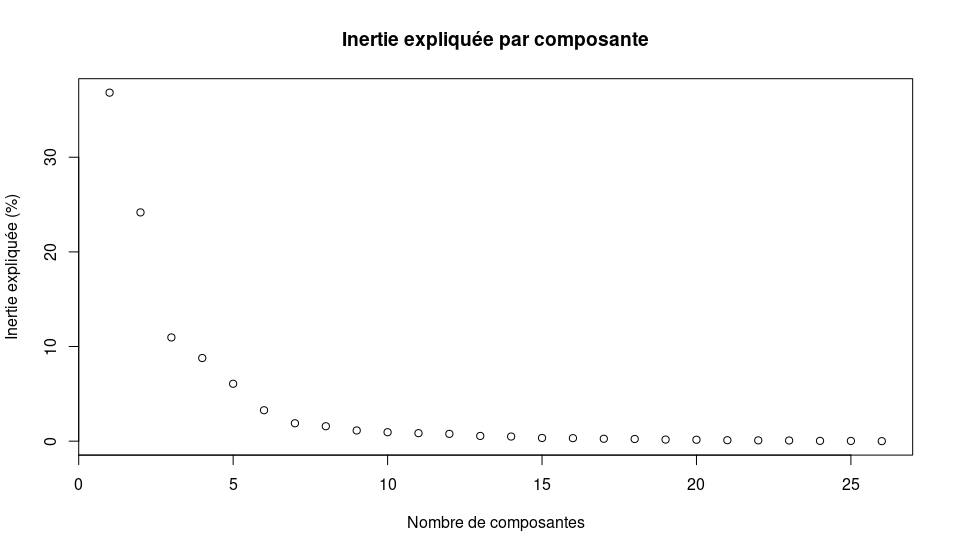
\includegraphics[scale = 0.32]{./doc/plot-inertie-par-composantes.png}
		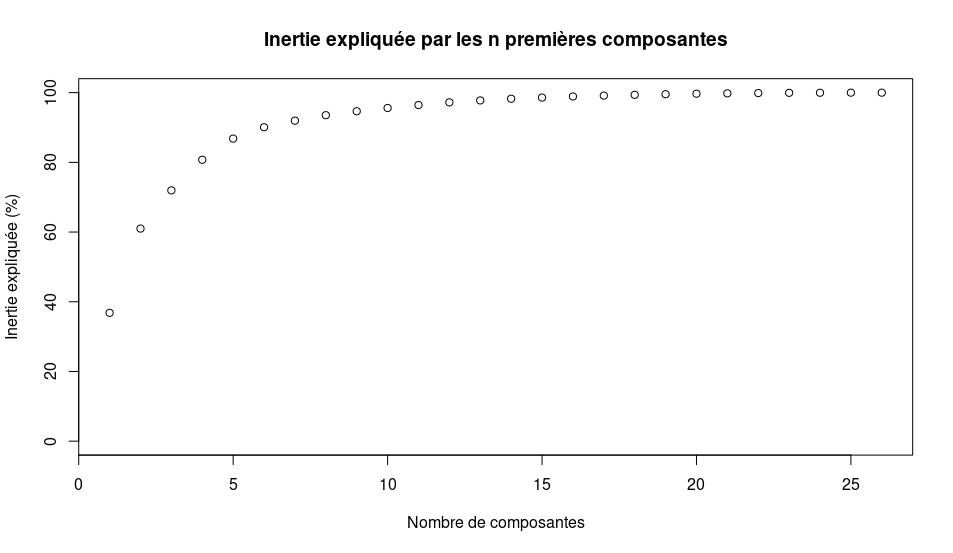
\includegraphics[scale = 0.32]{./doc/plot-inertie-n-composantes.png}
	\end{center}
\end{figure}

On constate que les deux premières composantes, bien qu'insuffisantes pour expliquer complètement les différences entre tous les points, permettent d'expliquer plus de 60\% de l'inertie. Il peut donc être intéressant d'afficher les points en fonction de ces composantes.
\begin{figure}[h]
	\begin{center}
		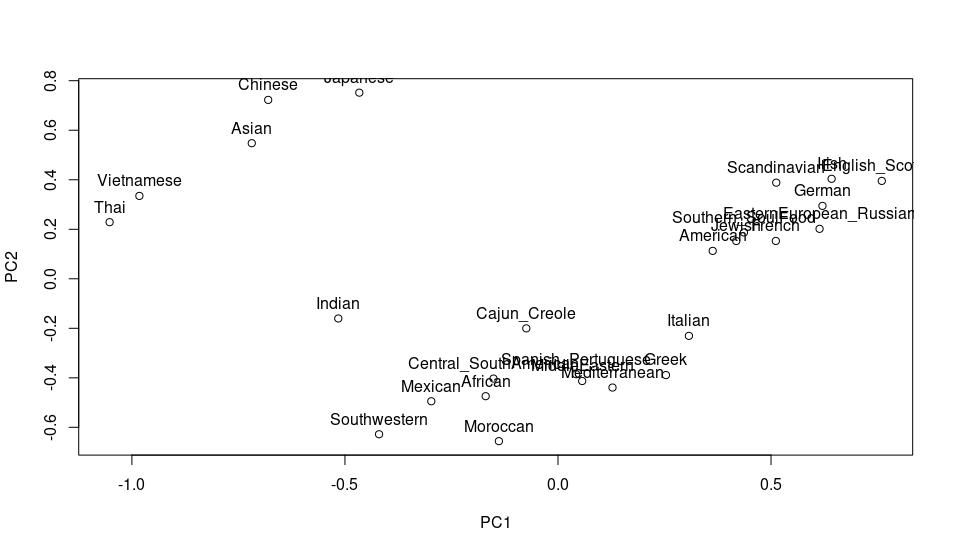
\includegraphics[scale = 0.32]{./doc/plot-recettes-composantes-1-2.png}
	\end{center}
\end{figure}

Par ce simple graphique on constate déjà certains regroupements entre les recettes des différents pays, avec trois groupes principaux qui ressortent. Grossièrement on a les recettes des pays asiatiques, des pays occidentaux et des pays méditerranéens. Ces deux composantes sont cependant insuffisantes à expliquer l'ensemble des subtilités de ces données, 6 composantes sont nécessaire pour expliquer 90\% de l'inertie.

On peut par exemple être surpris par la proximité entre les recettes des pays d’Amérique centrale et méditerranéens ou africains. En effet cette proximité disparaît si l'on affiche cette fois les points suivant les composante 1 et 3.
\begin{figure}[h]
	\begin{center}
		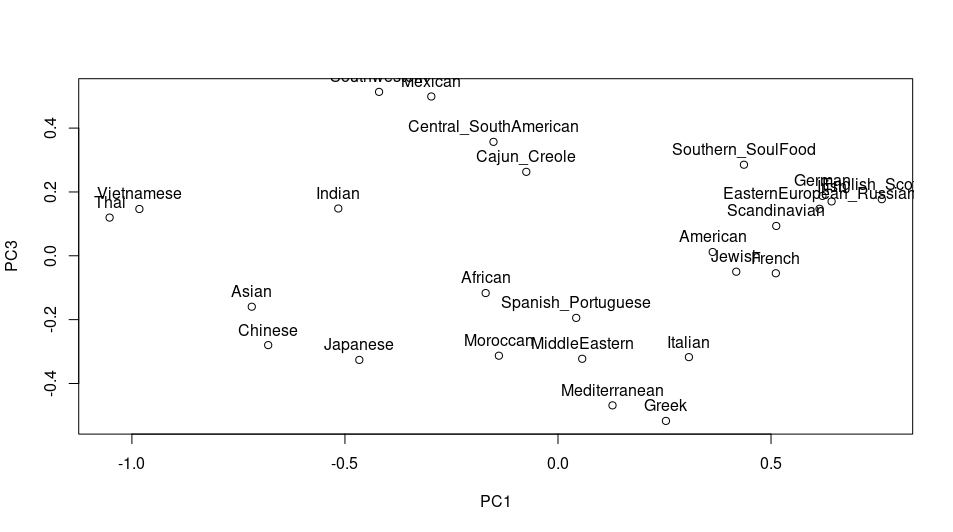
\includegraphics[scale = 0.32]{./doc/plot-recettes-composantes-1-3.png}
	\end{center}
\end{figure}

Une projection des anciens axes sur les nouveaux

\begin{figure}[h]
	\begin{center}
		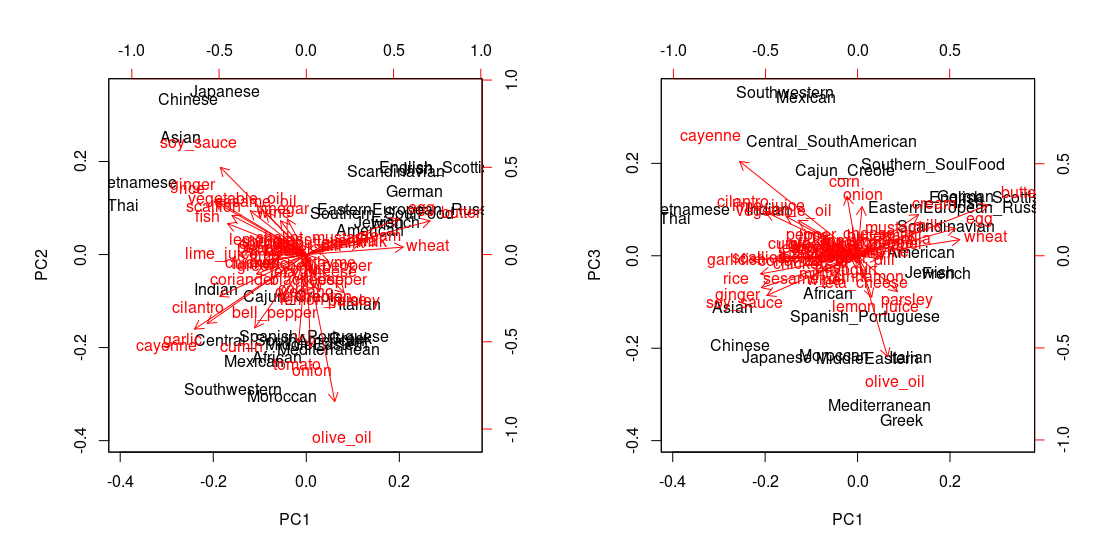
\includegraphics[scale = 0.32]{./doc/biplot-recette-pays.png}
	\end{center}
\end{figure}

\section{Analyse ascendante hiérarchique}
Nous avons choisi la méthode de Ward. Le critère de Ward est un critère d'inertie qui représente l'inertie inter-classe de deux classes quand nous faisons une fusion entre ces deux classes, donc en minimisant ce critère, nous pouvons obtenir une optimisation locale. Comme la distance n'est pas en carré, nous avons choisi Ward.D2 pour l'argument de méthode.
\begin{figure}[h]
	\begin{center}
		\includegraphics[scale = 0.32]{./doc/plot-CAH.png}
	\end{center}
\end{figure}

\section{K-Means}

En premier lieu on utilise une méthode du coude pour déterminer combien de centres il serait judicieux de choisir.

\begin{figure}[h]
	\begin{center}
		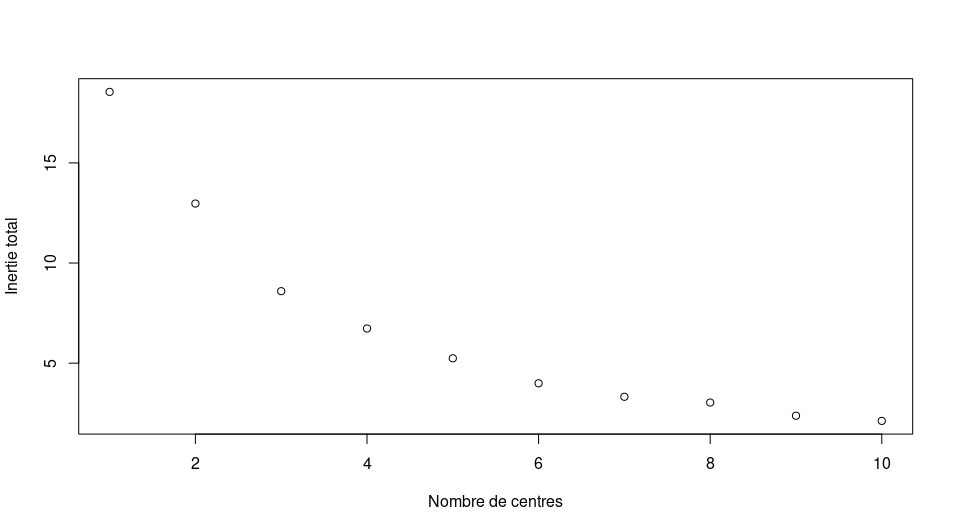
\includegraphics[scale = 0.32]{./doc/plot-kmeans-mininertie.png}
	\end{center}
\end{figure}

Ce graphe ne révèle pas de manière très net le nombre de groupes à sélectionner, on constate quand même qu'il y a une certaine rupture quand on dépasse les 3 groupes, et une autre moins évidente au delà de 5 groupes. 

\begin{figure}[h]
	\begin{center}
		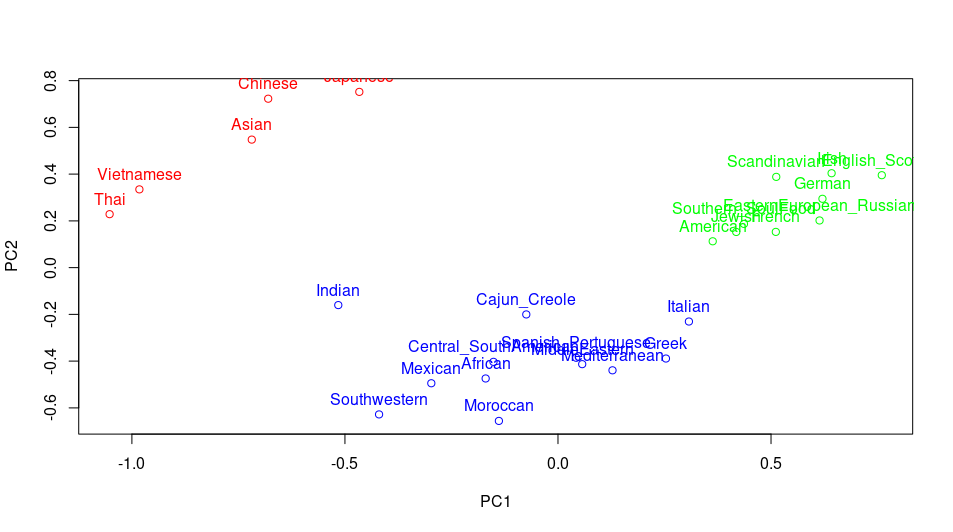
\includegraphics[scale = 0.32]{./doc/plot-kmeans-3.png}
	\end{center}
\end{figure}

En utilisant 3 groupes, on retrouve les groupes qui semblaient se dégager lors de l'ACP en affichant les points sur les deux composantes principales. 

\begin{figure}[h]
	\begin{center}
		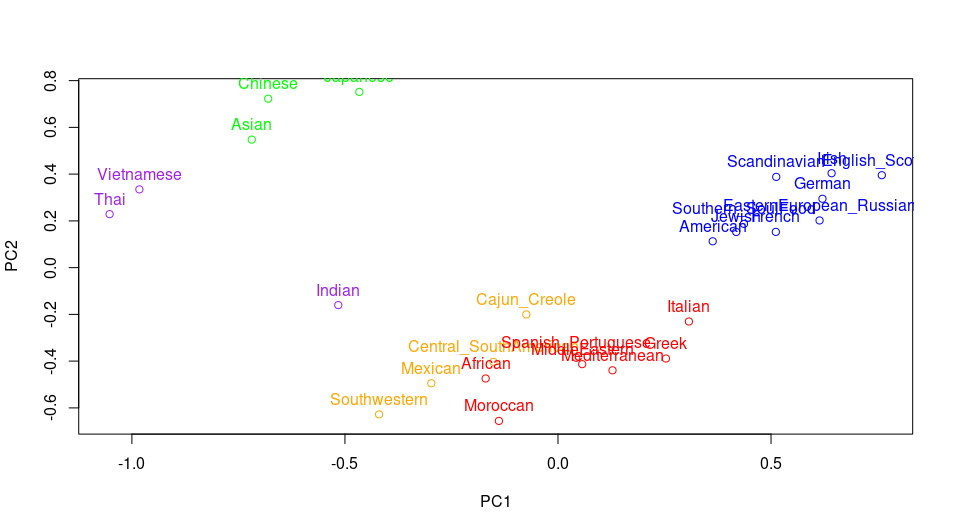
\includegraphics[scale = 0.32]{./doc/plot-kmeans-5.png}
	\end{center}
\end{figure}

La division en 5 groupes révèle une nouvelle division intéressante en séparant cette fois la cuisine des pays d’Amérique centrale des pays méditerranéens. Et en divisant les cuisines des pays asiatiques en deux groupes distincts.


\section{Comparaison}

On remarque très nettement, que ce soit en observant les données par rapport aux composantes principales obtenues avec l'ACP, à partir de l'analyse ascendante hiérarchique ou encore par l'algorithme des K-Means que les données semblent se regrouper en fonction de la situations géographique des pays étudiés. Cela semble tout à fait cohérent et c'est ce à quoi on pouvait s'attendre.
Les plats des différents pays sont généralement basés sur les aliments locaux, et plus des pays sont proches plus ces aliments seront susceptibles d'être similaires. Ainsi des traditions culinaires se sont développées sur la base de ces ingrédients, c'est pourquoi il est plus fréquent de trouver de la sauce soja dans les plats chinois et japonais que dans les plats français et allemands et inversement pour le blé.
De plus les recettes sont issues des traditions culinaires et culturelle, qui sont également influencées par la proximité territoriale des régions. Que ce soit par le commerce ou par un mélange de cultures cela a également un impact sur l'alimentation d'une population. Cette aspect culturel de la cuisine explique également la forte similarité observable entre les recettes de pays pourtant très éloignées. On peut citer l'Amérique du Nord, malgré sa distance de l'Europe, les recettes apparaissent ici très similaires. On peut associer ça à sa colonisation par l'Europe qui y a imposé sa culture.


\section{Analyse descriptive}

En chargeant les données, nous pouvons voir que ce jeu de données contient 2000 recettes et l'utilisation de 50 ingrédients d'une recette. Le chiffre 1 représente qu'il y a cet ingrédient dans la recette et 0 sinon. Les recettes viennent de 26 pays ou régions que nous avons vu précédemment.\\
\indent Nous pouvons voir que la répartition des recettes est inégale, c'est pourquoi nous ne pouvons pas les agréger simplement par la somme ou la moyenne dans les questions suivantes.

\begin{figure}[h]
	\begin{center}
		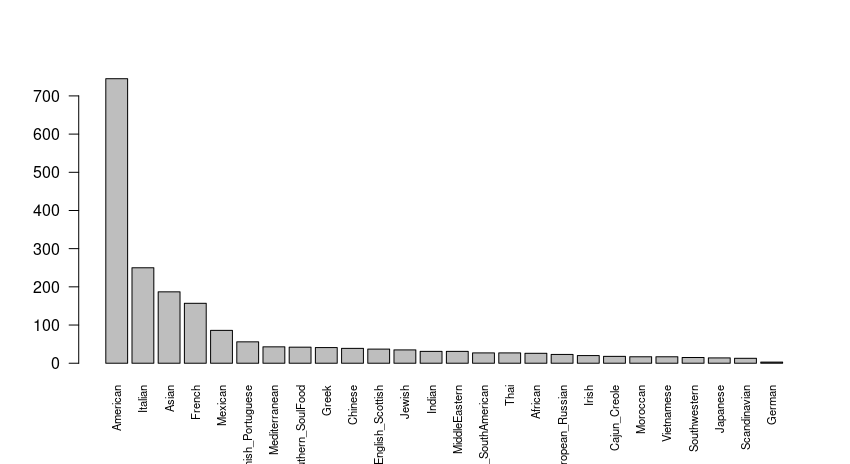
\includegraphics[scale = 0.32]{./doc/nombre-recettes.png}
	\end{center}
\end{figure}

\section{Similarité - Dissimilarités}

On traite ici un tableau de données binaires et on ne s’intéresse qu'aux ingrédients, on choisit donc d'utiliser une méthode de calcul de similarités binaire adapté à ce genre de calcul. Avec la distance de Jaccard, on peut comparer les membres de deux ensembles pour voir quels membres sont partagés entre deux ensembles et lesquels sont distincts. De plus la répartition des origines des recettes est très inégale dans ce jeu de données, les méthodes binaires permettent de palier naturellement à ce problème.


\section{Classification ascendante hiérarchique}

\begin{figure}[h]
	\begin{center}
		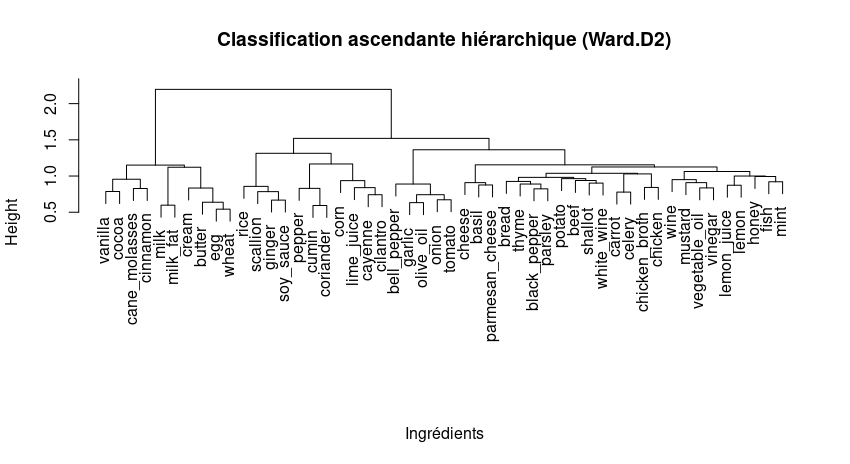
\includegraphics[scale = 0.45]{./doc/plot-hclust-ingredients.png}
	\end{center}
\end{figure}


\section{K-Médïodes}

\begin{figure}[h]
	\begin{center}
		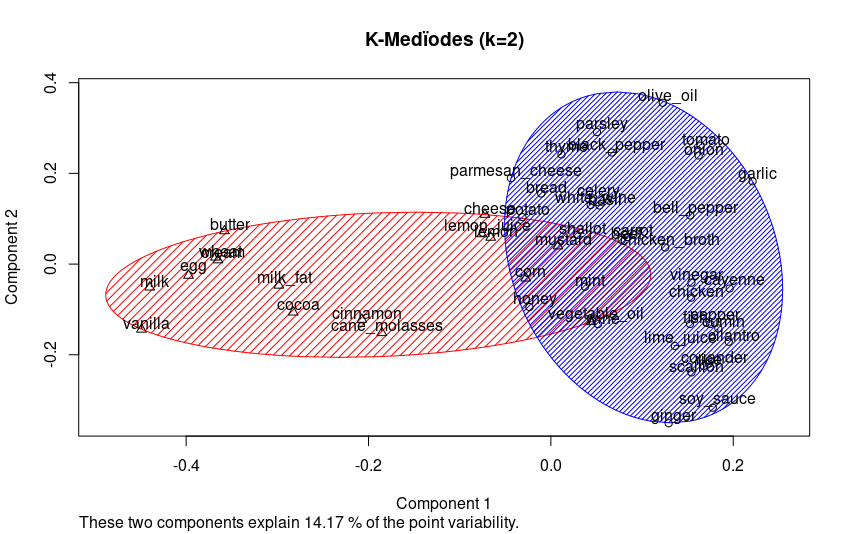
\includegraphics[scale = 0.45]{./doc/kmediodes-2.png}
		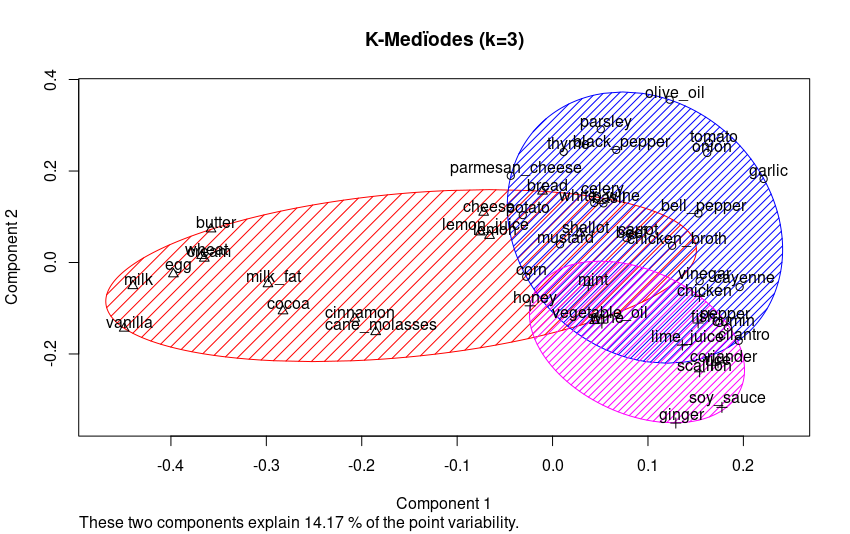
\includegraphics[scale = 0.45]{./doc/kmediodes-3.png}
		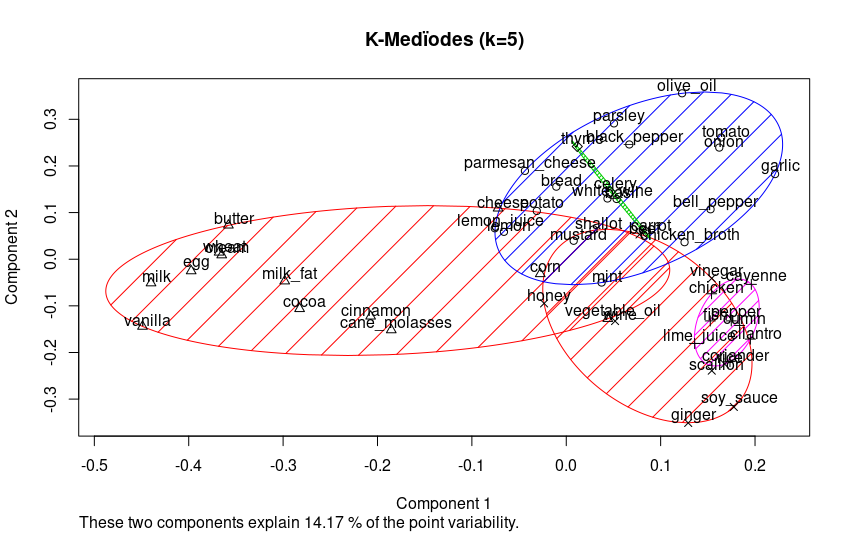
\includegraphics[scale = 0.45]{./doc/kmediodes-5.png}
		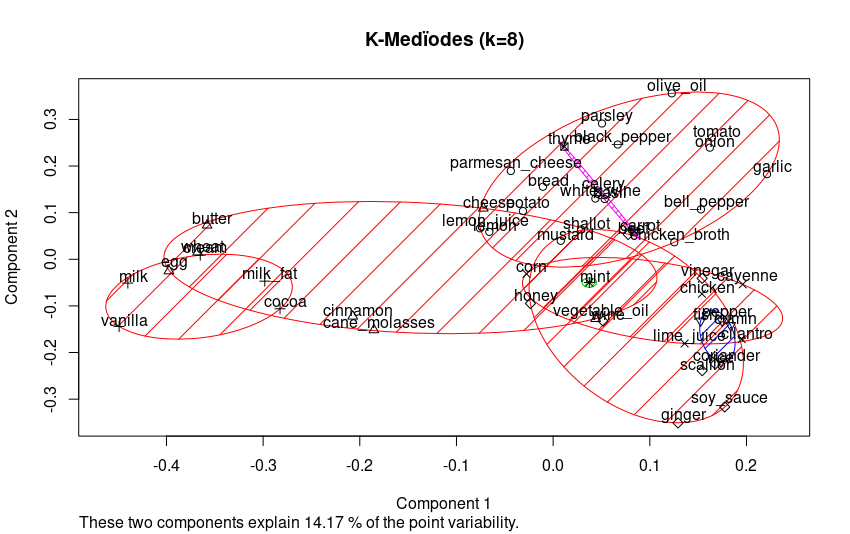
\includegraphics[scale = 0.45]{./doc/kmediodes-8.png}
	\end{center}
\end{figure}


\chapter{K-Means Adaptatif}

Le K-Means clustering est une méthode assez simple et performante pour la partition des données. Mais la méthode K-Means est limité à une utilisation sur des données distribuées de manière sphérique. Car elle se base sur la distance euclidienne pour calculer effectuer ses regroupements. Afin de palier à ce défaut, on peut remplacer la distance euclidienne par la distance de Mahalanobis, qui permet de tenir compte de la répartition des données.

\section{Données synthétiques}

Les jeux de données synthétiques qui sont mis à notre disposition sont constitués de deux groupes distincts. Ces deux groupes sont identiquement répartis entre les différents jeux de données. Seul leur proximité l'un de l'autre varie. Dans le premier cas ils sont distinctement séparés, dans le second légèrement plus proches, et dans le dernier ils sont en grande partie mélangés.

\begin{figure}[h]
	\begin{center}
		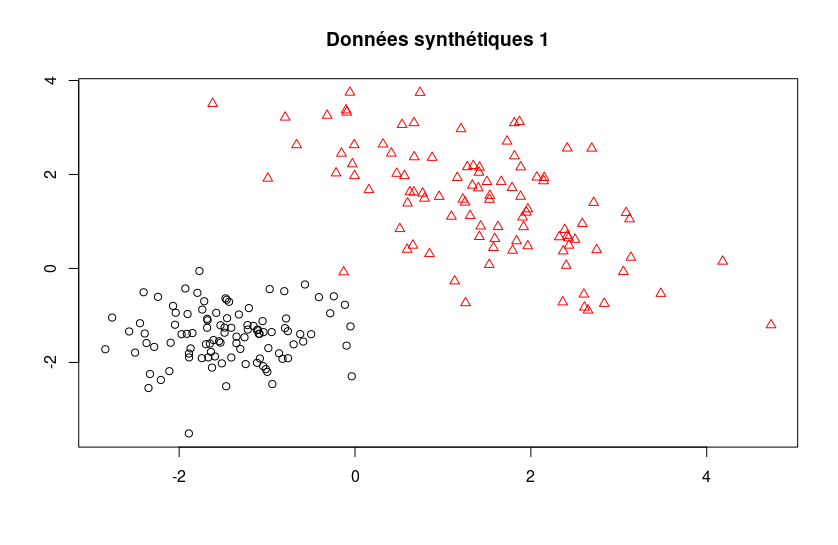
\includegraphics[scale = 0.22]{./doc/synt-1-reel.png}
		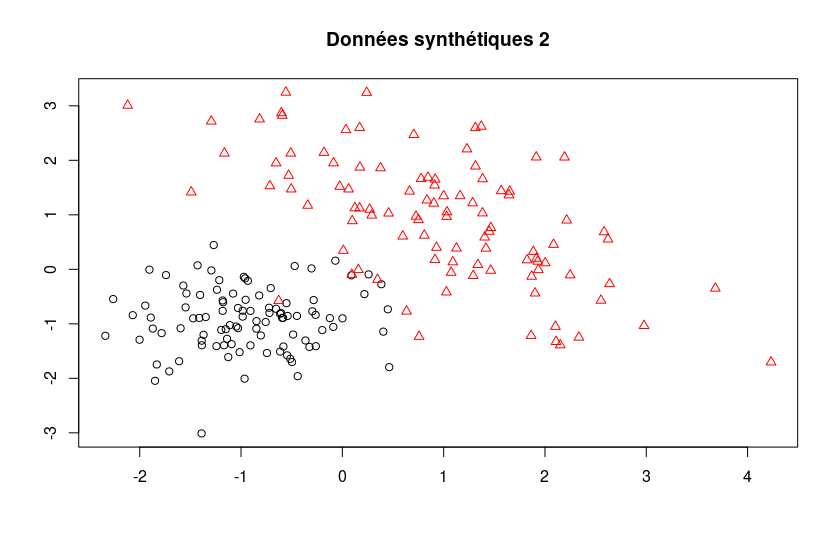
\includegraphics[scale = 0.22]{./doc/synt-2-reel.png}
		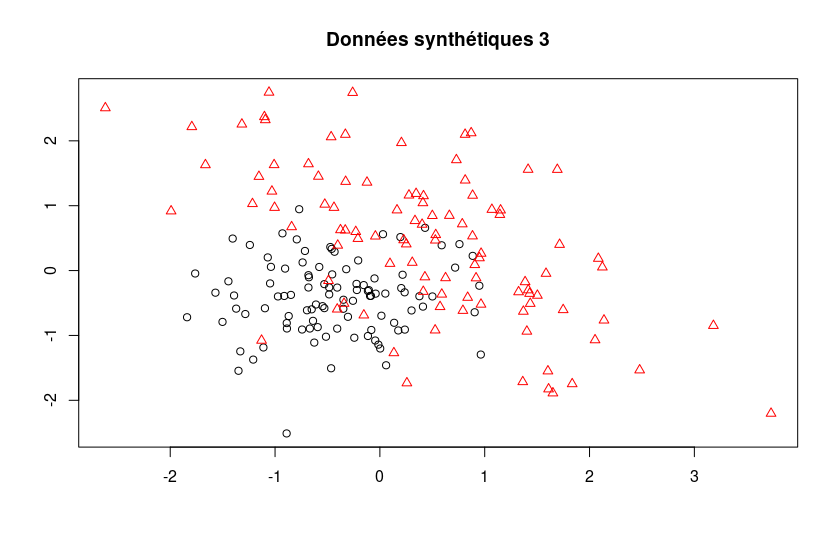
\includegraphics[scale = 0.22]{./doc/synt-3-reel.png}
	\end{center}
\end{figure}

On constate également que leur répartition est plutôt elliptique, l'algorithme des K-means adaptatifs pourrait donc s'avérer plus efficace que l'algorithme des k-means classique.

\subsection*{$1^{er}$ Jeu de données}

\begin{figure}[h]
	\begin{center}
		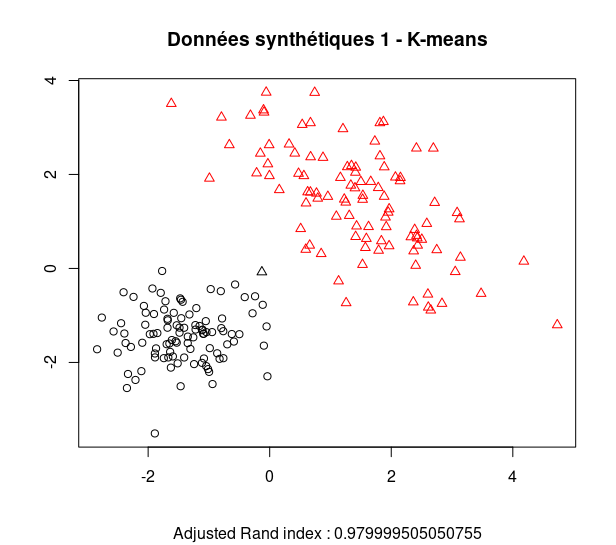
\includegraphics[scale = 0.35]{./doc/synt-1-k.png}
		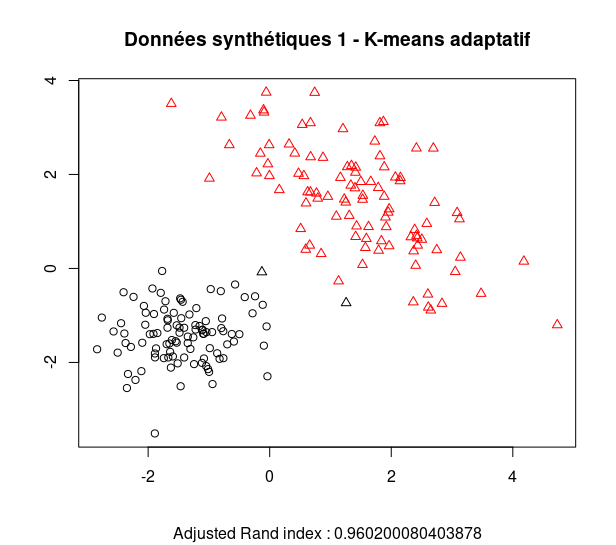
\includegraphics[scale = 0.35]{./doc/synt-1-ka.png}
	\end{center}
\end{figure}


\subsection*{$2^{nd}$ Jeu de données}

\begin{figure}[h]
	\begin{center}
		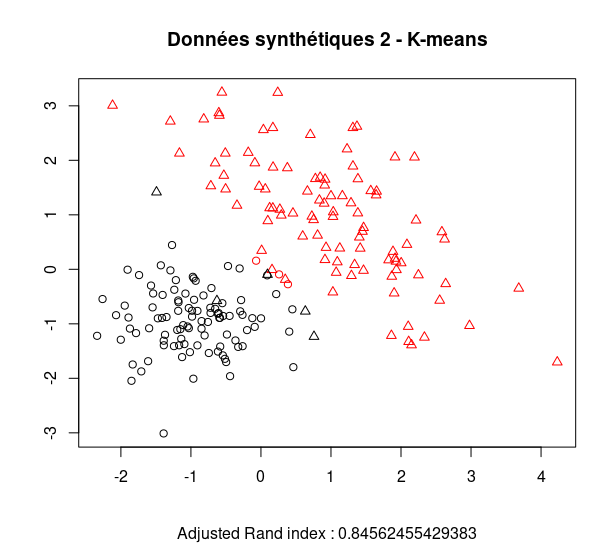
\includegraphics[scale = 0.35]{./doc/synt-2-k.png}
		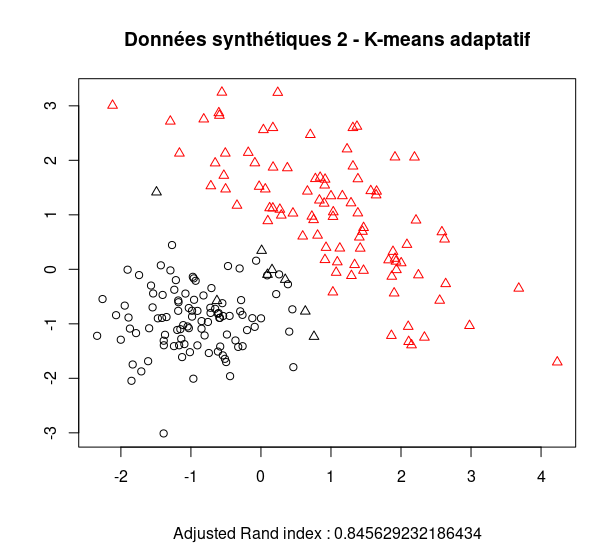
\includegraphics[scale = 0.35]{./doc/synt-2-ka.png}
	\end{center}
\end{figure}

Les deux algorithmes donnent des résultats très proches de la réalité dans ces deux cas. Le second cas est cependant un peu plus dur à traiter et les résultats sont un peu moins bons.


\subsection*{$3^{eme}$ Jeu de données}

Pour le troisième jeu de données les données sont bien plus mélangées, et il est évident qu'il n'est pas possible de les distinguer parfaitement les deux groupes avec ces deux axes seulement. Il est tout de même intéressant de confronter les deux méthodes dans cette situation.

\begin{figure}[h]
	\begin{center}
		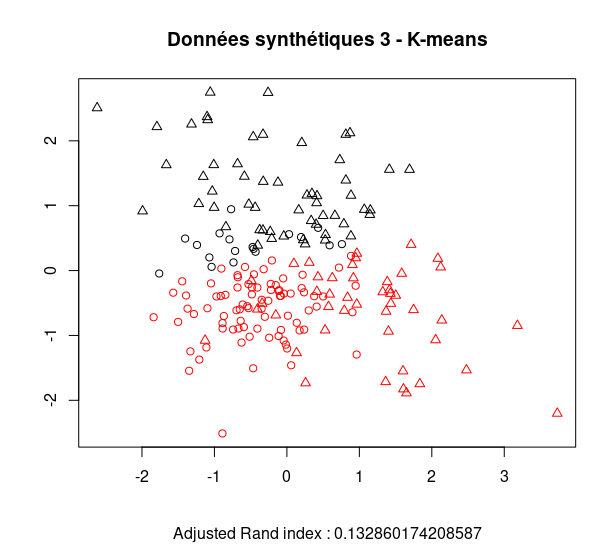
\includegraphics[scale = 0.35]{./doc/synt-3-k.png}
		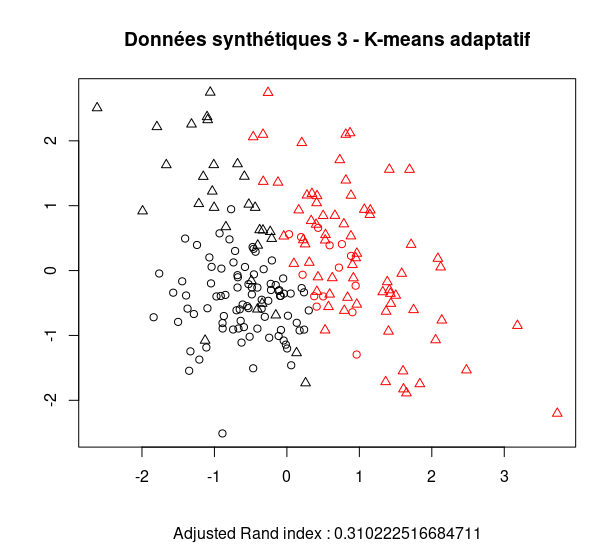
\includegraphics[scale = 0.35]{./doc/synt-3-ka.png}
	\end{center}
\end{figure}

\pagebreak
L'algorithme des K-means à distances adaptatives est largement plus performant dans cette situation que la version classique. Car celui-ci peut s’adapter à la répartition des données et ne requière pas que celle-ci soient sphérique. Les graphes suivants illustrent cette notion, seul le rayon des cercles peut changer en utilisant K-means, avec les distances adaptatives on peut avoir à faire à des ellipses de toutes formes.

\begin{figure}[h]
	\begin{center}
		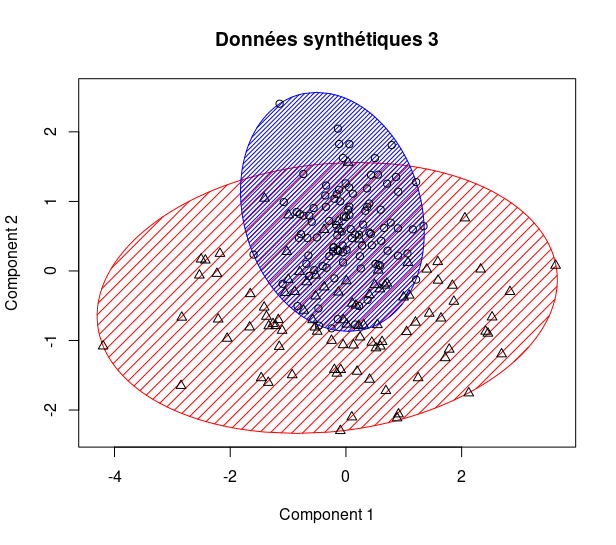
\includegraphics[scale = 0.22]{./doc/hclust-synt-3.png}
		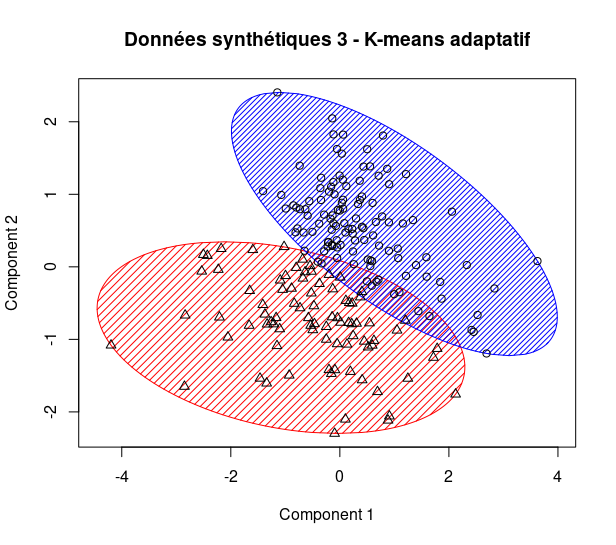
\includegraphics[scale = 0.22]{./doc/hclust-synt-3-ka.png}
		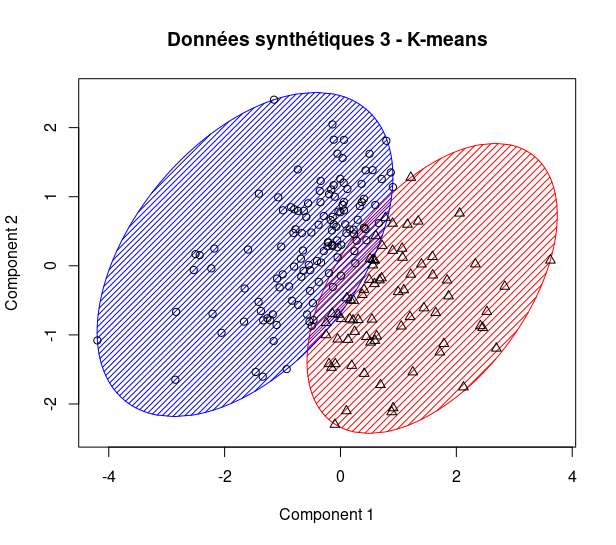
\includegraphics[scale = 0.22]{./doc/hclust-synt-3-k.png}
	\end{center}
\end{figure}

\tiny{Ici les axes sont les composantes principales de la matrice X donc les cercles sont légèrement déformés}

\newpage

\section{Iris}

\subsection*{Partitions pour k = 2,3,...,5}
\begin{figure}[h]
	\begin{center}
		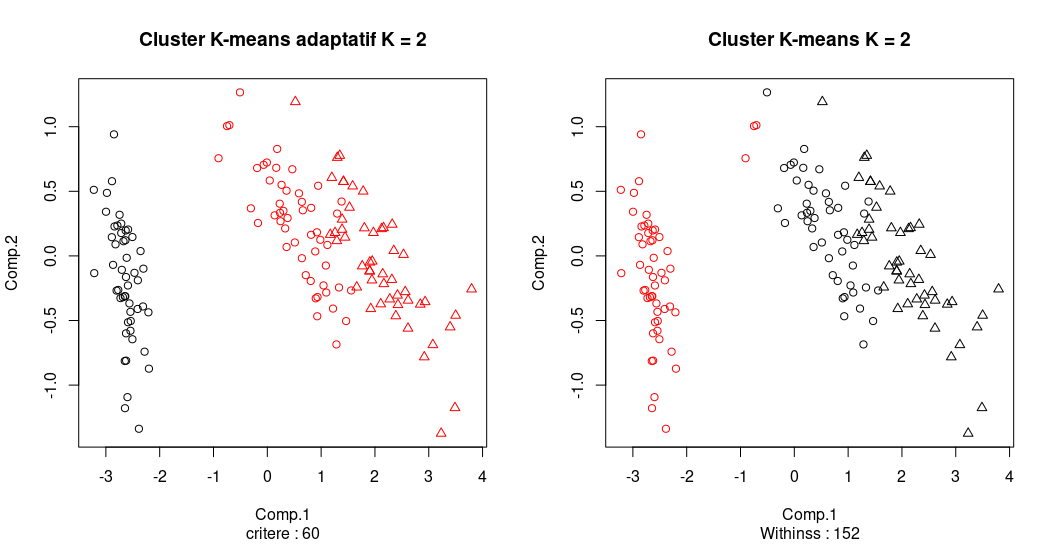
\includegraphics[scale = 0.21]{./doc/iris-ks-2.png}
		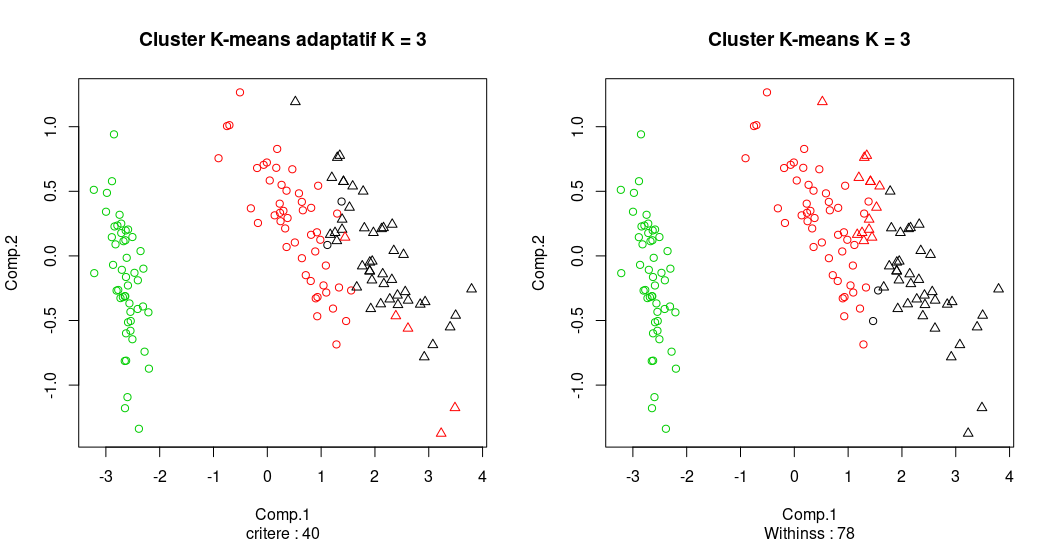
\includegraphics[scale = 0.21]{./doc/iris-ks-3.png}
	\end{center}
\end{figure}
\begin{figure}[h]
	\begin{center}
		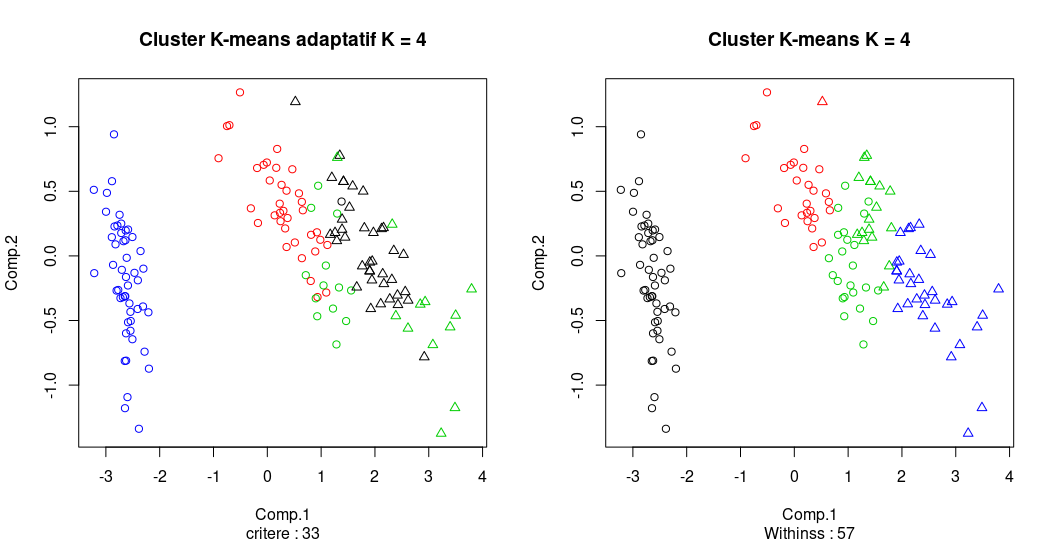
\includegraphics[scale = 0.21]{./doc/iris-ks-4.png}
		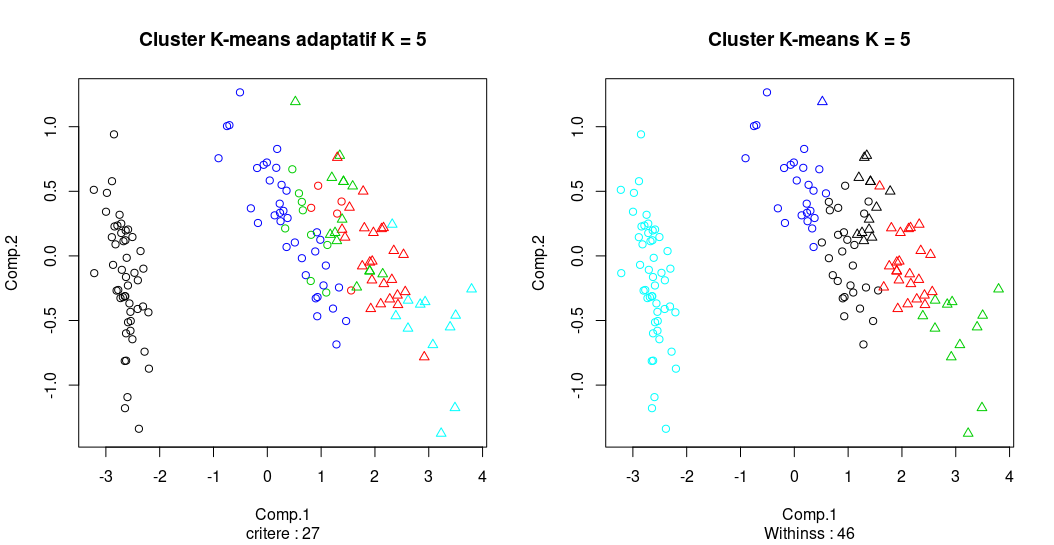
\includegraphics[scale = 0.21]{./doc/iris-ks-5.png}
	\end{center}
\end{figure}

Pour K=1 la valeur du critère optimisé est de 125 pour K-means adaptatif et de 681 pour k-means classique.
En calculant cette valeur pour chaque k compris entre 1 et 6 on obtiens le graphe ci-dessous. On peut en déduire que k-means classique est plus pertinent pour k=2 et que k-means adaptatif l'est pour k=3.

\begin{figure}[h]
	\begin{center}
		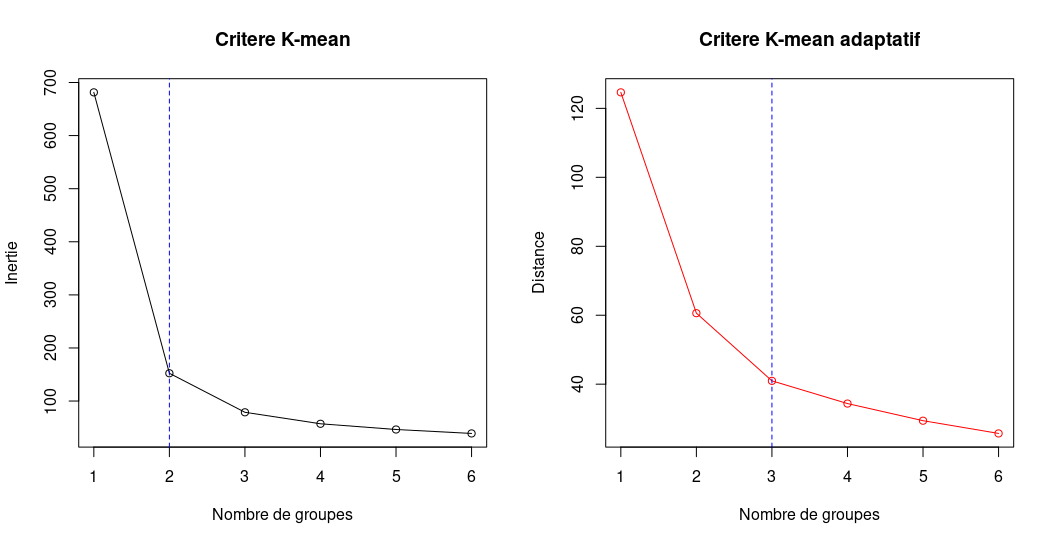
\includegraphics[scale = 0.42]{./doc/kmvkma-iris.png}
	\end{center}
\end{figure}

On comprends les suppositions précédentes en observant les résultats obtenus pour k = 2 et k = 3 et en les comparant aux espèces des iris que l'on étudie. La version classique de K-means permet de différencier les Setosa des autres iris, mais ne permet pas de distinguer les Versicolor des Virginica. Comme on peut le constater sur les partitions établies plus haut avec K = 2 les groupes sont pertinents, mais pas avec k = 3. En revanche avec distances adaptatives, l'algorithme des K-means distingue nettement les trois types d'espèces. C'est ici aussi dû a la répartition des données qui n'est pas adaptée à une utilisation de K-means classique.




\newpage
\section{Spam}
Le jeu de données spam de mail est composé de 4601 lignes et 58 colonnes. Une ligne représente un mail. Les premières 48 variables sont les mots, et la variable 49 jusqu'à la variable 54 sont les caractères comme ";" et "(". Les valeurs dans le tableau pour les 54 premiers colonnes sont les pourcentages d'apparition des mots ou des caractères au sein d'un mail. Puis la colonne 55 est la moyenne du longueur des séquences ininterrompues des lettres capitales; la colonne 56 est la plus long séquence ininterrompue des lettres capitales; la colonne 57 est la somme du longueur des séquences ininterrompues des lettres capitales. La dernière colonne indique ce mail est spam (1) ou pas (2).\\

Et contrairement aux applications précédentes, la séparation des données assez floue, et les la répartition non sphérique. L'algorithme des K-means classique ne devrait donc pas être utilisable ici.

\begin{figure}[h]
	\begin{center}
		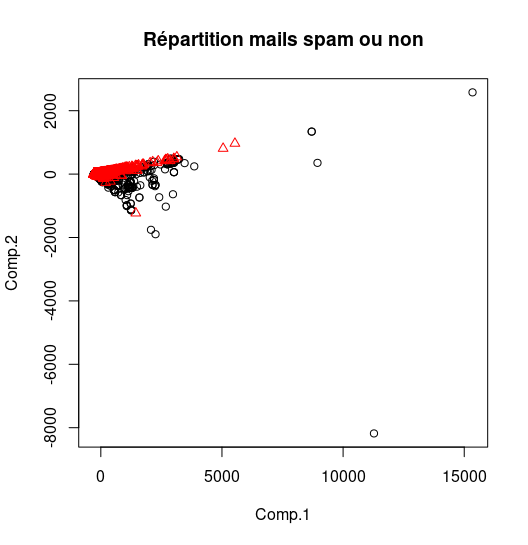
\includegraphics[scale = 0.30]{./doc/plot-c12-vrai-spam.png}
		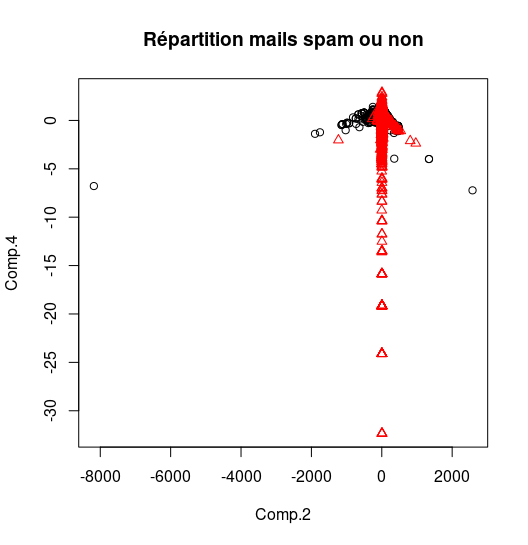
\includegraphics[scale = 0.30]{./doc/plot-c24-vrai-spam.png}
	\end{center}
\end{figure}

Nous avons tout d'abord essayé d'appliquer l'algorithme des K-means adaptatif sur les données telles quelles, mais les résultats n'étaient absolument pas fiables. Les deux types de mails ne semblaient pas se distinguer. Nous avons donc décidé de faire un pre-traitement des données à l'aide d'une acp, et de ne conserver que les premières valeurs afin d'obtenir de meilleurs résultats sans certains facteurs indésirables. Les deux premières composantes expliquent plus de 95\% de l'inertie, mais une classification sur ces facteurs ne donne pas non plus de résultats exploitable. L'inertie expliqué par les axes ne semble donc pas être une bonne base pour choisir les composantes à utiliser. Ainsi nous avons cherché avec quelle combinaison d'axes on obtenait les meilleurs résultats.

\begin{figure}[h]
	\begin{center}
		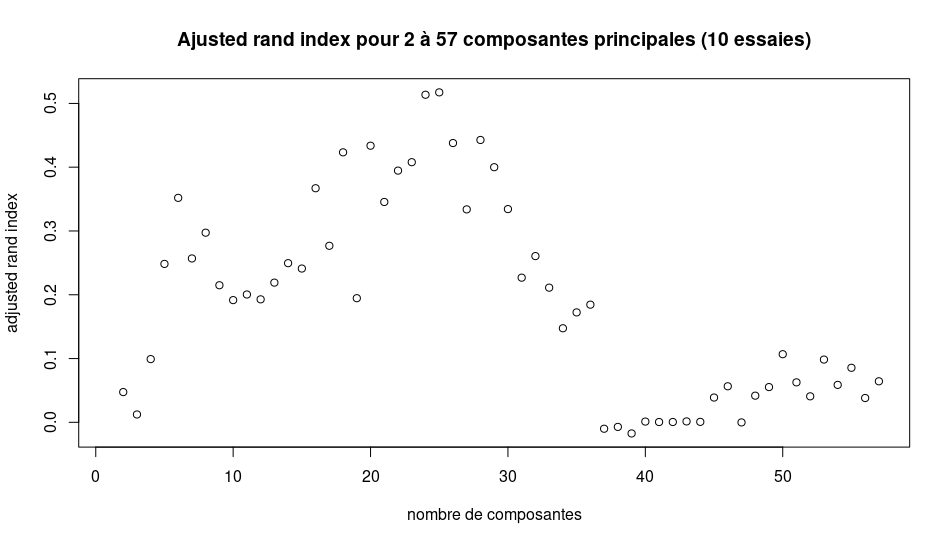
\includegraphics[scale = 0.30]{./doc/plot-ari-2-57.png}
		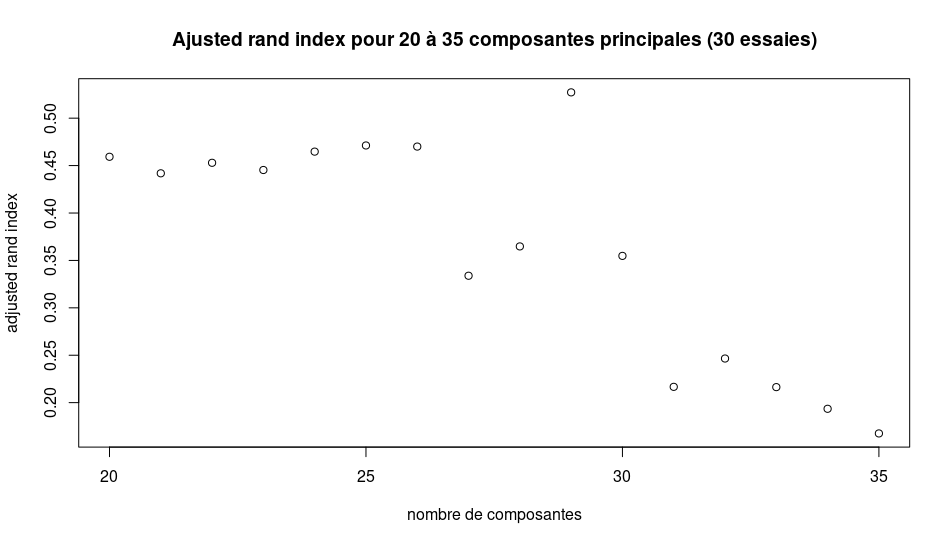
\includegraphics[scale = 0.20]{./doc/plot-ari-20-35.png}
		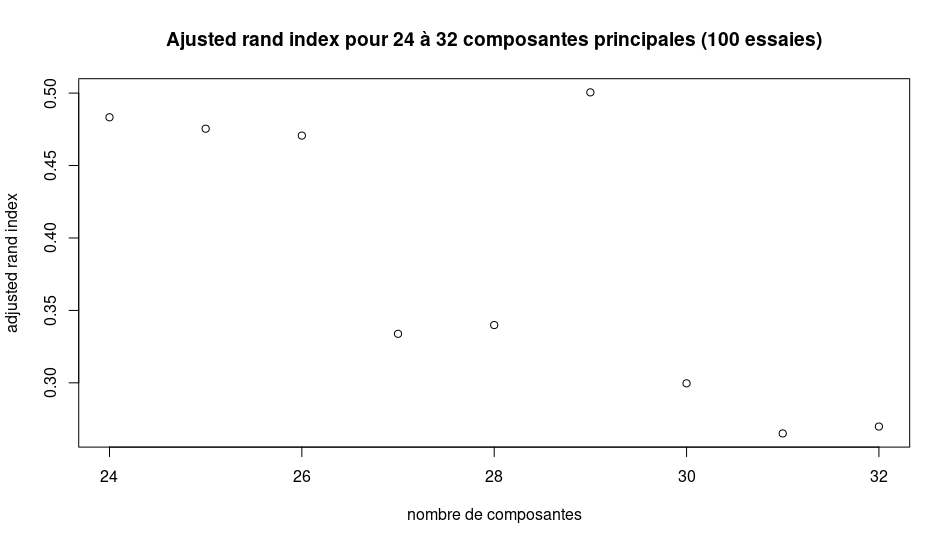
\includegraphics[scale = 0.20]{./doc/plot-ari-24-32.png}
	\end{center}
\end{figure}

\pagebreak
En appliquant l'algorithme des K-means adaptatif sur les n premières composantes nous avons pu conclure que le meilleur indice de Rand était obtenu lorsque l'on utilisait les 29 premières composantes de l'ACP. Celui-ci avoisine dans les meilleurs des cas les 0.55, on obtiens les figures suivantes :


\begin{figure}[h]
	\begin{center}
		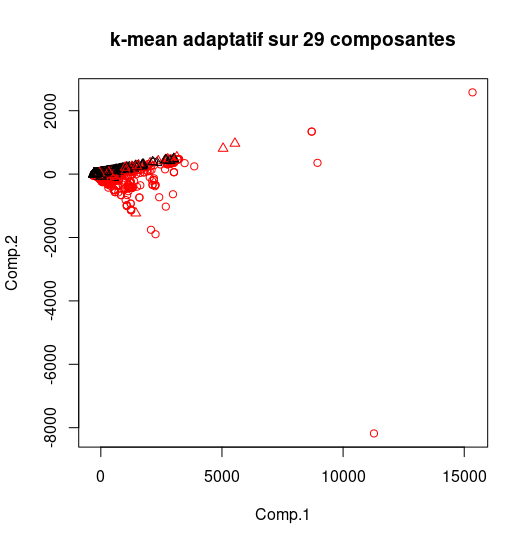
\includegraphics[scale = 0.40]{./doc/spam-comp-1-2.png}
		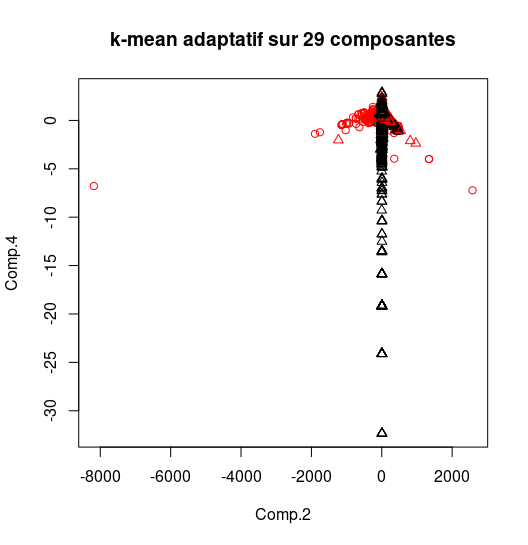
\includegraphics[scale = 0.40]{./doc/spam-comp-2-4.png}
	\end{center}
\end{figure}

En revanche l'algorithme des K-means classique n'est absolument pas adapté à ce type de problème comme nous le supposions initialement. L'indice de Rand calculé dans les mêmes conditions ne dépasse jamais les 0.1.




\chapter*{Annexe}
\lstinputlisting[firstline=0, lastline=108]{./doc/partie-1.R}


\end{document}
